\documentclass[1p]{elsarticle}

\usepackage{lineno,hyperref}
\modulolinenumbers[5]
\usepackage[utf8]{inputenc}
\usepackage[spanish]{babel}
\usepackage{amsmath}
\usepackage{graphicx}
\usepackage{amsfonts}
\usepackage{amssymb}
\newtheorem{thm}{Teorema}
\newtheorem{lem}[thm]{Lema}
\newdefinition{rmk}{Remark}
\newproof{pf}{Demostración}
\newproof{pot}{Demostración del Teorema \ref{thm2}}
%%\bibliographystyle{IEEEannot}

%% `Elsevier LaTeX' style
\bibliographystyle{elsarticle-num}
%%%%%%%%%%%%%%%%%%%%%%%
\usepackage{setspace}  
\begin{document}

\begin{frontmatter}

\title{A review of the paper: \textit{Inherent directionality explains the lack of feedback loops in
	empirical networks} }

%% Group authors per affiliation:
\author{Rubén Hurtado, Bartolomé Ortiz, Cristina Seva}
\address{Master en Física y Matemáticas\\ Universidad de Granada\\10/06/2018}

\begin{abstract}
This work is a brief revision and study about a paper called: \textbf{Inherent directionality explains the lack of feedback loops in empirical networks} written by \textit{Virginia Domínguez García, Simone Pigolotti and Miguel A. Muñoz}  . Our aim is to present its mains results, some technical highlights related to the mathematical and physical advances, and reproduce a minor result using our own methods. It will be analized its implications and future research too. Althought this work is merely a revision it could be useful as a source of code to reproduce some of the results.
\end{abstract}

\begin{keyword}
 \texttt{complex networks} \sep \texttt{mathematics}\sep \texttt{complexity} \sep \texttt{graph theory}

\end{keyword}

\end{frontmatter}
\setlength\parindent{0pt}
\linenumbers

\section{Introducción}
\spacing{1.5}
El objetivo de este trabajo es presentar el artículo seleccionado \cite{arti}, de manera que expondremos sus principales descubrimientos, así como algunas notas sobre los procedimientos que en él se presentan. 

Tras esto, vamos a realizar un pequeño intento de simulación para intentar reproducir algunos de los resultados que aparecen en el articulo.

Finalmente, para cerrar nuestro trabajo, hablaremos un poco sobre las conclusiones obtenidas de este y sobre posibles vías para avanzar.

\section{Review del artículo}
\spacing{1.5}
El artículo muestra una serie de resultados que relacionan la direccionalidad inherente al sistema complejo (representado mediante grafos) con la ausencia de ciclos que se retroalimenten dentro de este grafo. 
Para continuar vamos a dar una pequeñas nociones sobre los elementos fundamentales del artículo:
\begin{itemize}
	\item \textbf{Direccionalidad inherente}: hablamos de direccionalidad inherente a un sistema complejo cuando todos los nodos se pueden ordenar en un eje unidimensional, de tal manera que los enlaces apuntan desde valores bajos a altos de sus coordenadas en dicho eje. 
	
	Como bien se apunta en \cite{arti}, la existencia de esta direccionalidad está relacionada con la existencia de una estructura jerárquica dentro de nuestra red. Así, aunque la aplicación de los resultados es muy amplia, podemos relacionarlo directamente con la temática de redes tróficas que vimos en clase. 
	\item \textbf{Ciclo retroalimentado o feedback loop}: hablamos de ciclo retroalimentado de orden $k$ dentro de un grafo direccional, cuando nos referimos una sucesión cerrada de $k$ nodos (esto es, con el mismo nodo en primera y última posición), cuyo orden de aparición viene determinado por el camino que indica el sentido de las aristas que los conectan.
	\item \textbf{jerarquía} Hablamos de jerarquía en un grafo cuando 
	\item \textbf{ascents}
\end{itemize}

Debido al gran impacto de la existencia de feedback loops en la estabilidad dinámica del sistema, el artículo se centra en encontrar una herramienta predictiva para conocer, basándose en un solo parámetro $\gamma$, la fracción de ciclos de orden $k$ que también son ciclos retroalimentados. Se observa experimentalmente que esta fracción siempre es menor en redes con direccionalidad inherente que en redes aleatorizadas.

\subsection{Métodos}
Exponemos ahora la forma de obtener la herramienta predictiva descrita en el artículo.

Consideramos una red de $N$ nodos, y $L$ aristas e imaginamos que conocemos la fracción de ciclos retroalimentados de orden $k$: $F(k)$. Con ello , si asumimos la existencia de direccionalidad, se construye el modelo aleatorizando la direccionalidad de la siguiente manera: 
\begin{itemize}
	\item Se escoge un nodo. Con probabilidad $0<\gamma<1$ su arista apunta en la dirección inherente, i.e.; hacia los nodos de mayor jerarquía, y con probabilidad $1-\gamma$ apunta en sentido contrario.
\end{itemize}
Al parámetro $\gamma$ se le llama \textbf{parámetro de direccionalidad.}

Si ahora nos centramos en un ciclo de orden $k$ e imponemos una notación jerárquica para los nodos de este ciclo obtendríamos un total de $k!$ posibles ciclos. 

En general, la probabilidad de tener un ciclo retroalimentado dado un ciclo cualquiera dependerá del numero de ascensos $A(l,k)$.
Este numero cuenta cuántas permutaciones de la secuencia básica de longitud $k$ con $nodo_{i}<nodo_{i+1}$ se tienen para $l$ valores distintos de $i$. Para una secuencia no periódica, es decir, sin establecer ninguna relación entre $nodo_k$ y $nodo_1$
la solución a este problema está dada por los llamados números eulerianos.

 Sin embargo, como los ciclos que buscamos, al ser retroalimentados, están cerrados, se  generaliza el concepto de números de Euler para el caso periódico o cíclico. Es decir, necesitamos contar el número de ascensos en un ciclo cerrado genérico, lo que en el articulo se bautiza como los \textbf{numeros eulerianos cíclicos}, denotados por $A(l,k)$.
Con este interesante concepto en mente, los autores ya pueden desarrollar la expresión de la función buscada, necesitando ahora añadirle el parametro de direccionalidad:
$$F(k,\gamma)=\sum_{l=0}^{k}\frac{A(l,k)}{k!}[\gamma^l(1-\gamma)^{k-l}+\gamma^{k-l}(1-\gamma)^l]$$
Usando los procesos del material suplementario, la expresión puede aproximarse por :
$$F(k,\gamma)\approx 2exp\{\frac{k}{2}log[\gamma(1-\gamma)]+\frac{k}{24}log^2(\frac{\gamma}{1-\gamma})\}$$

Esta expresión es la que hemos usado para todas las partes replicadas de nuestra revisión.
Para concluir, presentamos en la gráfica \ref{h}, que también se puede ver en \cite{arti}, la relación entre el parámetro de forma y la fracción $F(k,\gamma)$

\begin{figure}
	\centering
	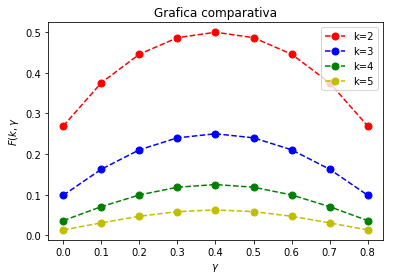
\includegraphics[width=12cm]{graf_1.png}
	\caption{$F(k)$ frente a $\gamma$, se puede observar el pico en $\gamma=1/2$}
	\label{h}
\end{figure}




\subsection{Algunos resultados a destacar}
Entrando en la parte de resultados, queremos destacar algunos de los que nos han parecido más relevantes.
\begin{itemize}
	\item La fracción de los ciclos de retroalimentación de cualquier longitud $k$ es mucho más pequeña en redes biológicas y ecológicas de lo que cabría esperar para cualquier otro grafo similar pero aleatorizado.
	\item El número total de ciclos de retroalimentación también se reduce 
	con respecto a las aleatorizaciones de red. Sin embargo, y esto es por lo que nos llamó la atención realizarlo en Twitter, estas tendencias no son tan evidentes para las redes socio-tecnológicas; mientras que todas las redes consideradas tienen una fracción más pequeña de bucles de retroalimentación que sus aleatorizaciones de direccionalidad, la red social de Twitter exhibe una mayor $F(k)$ que las aleatorizaciones.
	\item Por supuesto, el modelo desarrollado reproduce bastante bien las muestras experimentales obtenidas, que muestran un decaimiento exponencial de $F(k)$ conforme aumenta $k$.
\end{itemize}

Para observar gráficamente estos resultados podemos irnos a la gráfica \ref{h1}, donde hemos destacado la sección de redes tecnológicas. Antes, sin embargo debemos hacer una reseña sobre la información a encontrar:

 En la grafica se compara la fracción medida de los ciclos retroalimentados $F(k)$ con dos aleatorizaciones de la misma red. La primera, que llaman aleatorización de la direccionalidad (DR) - conserva las aristas existentes, pero aleatoriza completamente sus direcciones. La segunda, aleatorización de configuración (CR), aleatoriza tanto aristas como direcciones, pero preservando la conectividad de entrada y salida de cada nodo.
\begin{figure}
	\centering
	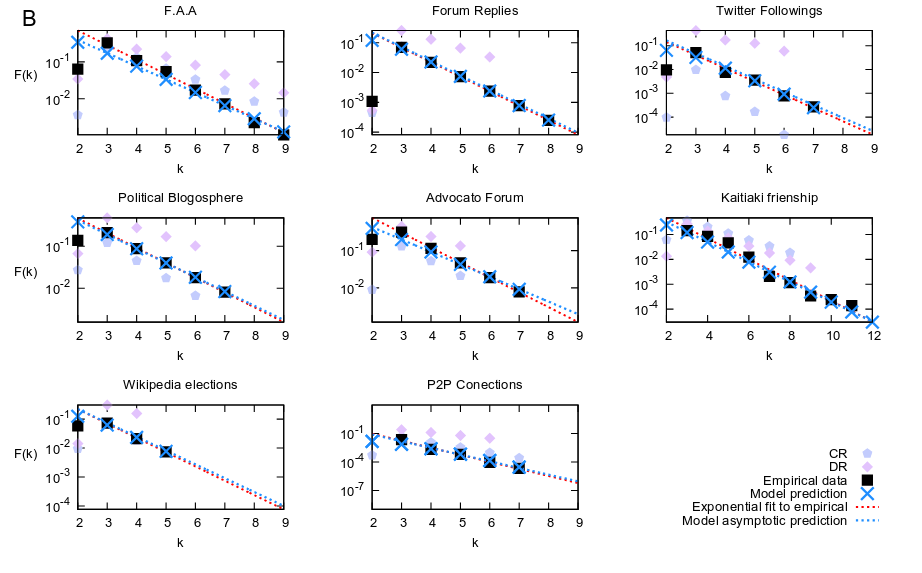
\includegraphics[width=15cm]{graf_2.png}
	\caption{Gráfico extraído del artículo donde resaltamos la parte de redes tecnológicas}
	\label{h1}
\end{figure}

Finalmente queremos resaltar el apartado sobre cómo información sobre nuevos nodos puede alterar lo que sabemos hasta ahora por las predicciones.

 Para probar la robustez
de su predicción, los investigadores simularon el efecto de desconocimiento sobre las redes que ya tenían,
eliminando una fracción de los enlaces al azar, y repitieron el análisis anterior. 

Aunque esta operación afecta claramente a la cantidad de enlaces, las conclusiones del modelo apenas varían, lo cual nos parece muy interesante. Incluso, cuando la cifra de nodos que se elimina está entre $20-$ y $50-$ podemos observar esta tendencia en la gráfica obtenida del material suplementario \ref{h4}
\begin{figure}
	\centering
	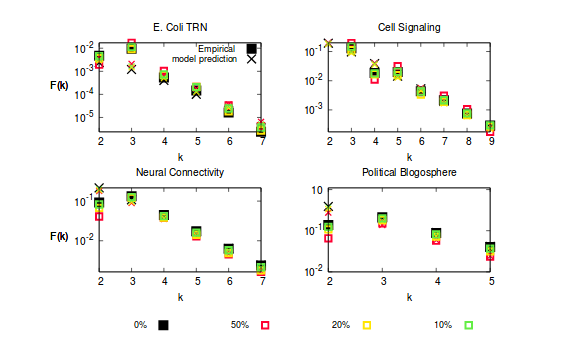
\includegraphics[width=15cm]{graf_3.png}
	\caption{Gráfico extraído del artículo donde resaltamos el impacto de los nodos o conexiones no observadas}
	\label{h4}
\end{figure}

\section{Intento de reproducción}
\spacing{1.5}

Escribir.

En particular nos centramos en la reproducción de redes en Twitter. En este caso estaríamos ante una predicción como la que se observa en la gráfica \ref{h2}.
\begin{figure}
	\centering
	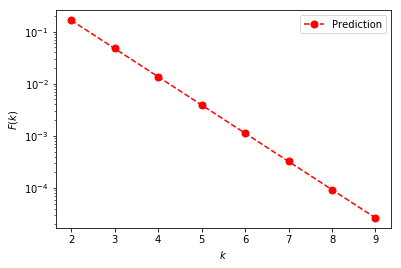
\includegraphics[width=9cm]{graf_4.png}
	\caption{Gráfico extraído del artículo donde resaltamos la parte de redes tecnológicas}
	\label{h2}
\end{figure}

\section{Conclusiones finales}
\spacing{1.5}
\section*{Referencias}
\spacing{1.5}
\bibliography{bibliograf}

\end{document}
